\section{Signal systematic uncertainties}
\label{sig_syst}
Systematics uncertainties due to the mismodel of the signal have been taken into account in the signal extraction and discussed in this section.
We distinguish between ``{\it shape}'' uncertainties, that affect the description of the peak in each category, ``{\it rate}'' uncertainties,
that change the total number of Higgs events expected, and ``{\it category migration}'' uncertainties, that migrates events from one category to the other.

\subsection{Shape Uncertainties}
Shape uncertainties affect the signal model in each category and process.
The peaky structure used to identify the Higgs boson resonance, is affected by muon momentum scale and resolution.
The momentum scale and resolution measurements provide corrected values for muon momentum such that data and MC matches.

\begin{itemize}
    \item {\bf Muon Scale}, it amounts up to ??? %% $1\text{\textperthousand}$
{\bf FIXME, implement and check values.}, of the muon momentum and its effect is to change the position of the peak with respect to its nominal value.
        %It has been observed that Kalman-Filter corrections have a better description of the muon momentum scale w.r.t. the Rochester corrections, making the
    \item {\bf Muon Resolution}, it amounts up to $10\%$ with rispect to its nominal value {\bf FIXME check correlations.}.
        It's effect is to enlarge the peak, changing therefore the amount of background in one effective signal, and allowing for a better/worse measurement of the signal strength (or upper limits).
\end{itemize}

Variation across the eigen-values of the measurements suggests that ... , {\bf FIXME}

\subsection{Category migration}
The following uncertainties are primarly responsible to category migrations across the bdt categorization, and rate uncertainty due to migration across the minimum requirements for entering the classification. It has been verified within the statistical power of the MC
that no major shapes distortions are present.

\begin{itemize}
    \item {\bf Jet Energy Scale}, after applying the jet energy corrections {\it Summer16\_23Sep2016AllV4 }, the energy scale of the jet is varied as a single nuisance parameter as provided by the JetMET group cite-JEC-FIXME fully correlated across the selected jet and the missing transverse energy. Due to VBF like classification this changes corresponds to yields variations, espetially  in the high sensitive categories, where it amounts up to $6\%$ in the  variations of the yields. This uncertainty is the dominant experimental uncertainty in the measurement,
    i.e. the uncertainty with the largest impact on the parameter of interest among the one listed;
    the full migration for the two dominant signal process (qqH and ggH) are reported in table~\ref{tab:jes}.
    \item {\bf Jet Energy Resolution}, the jet energy resolution can also induce category migration due to the non-linearly falling spectrum of the jet transverse momentum. It has a modest impact with respect to the scale and it amounts to up to few percent across the categories.
    \item {\bf Pileup Reweighting}, pileup reweighting procedure uses the ``minimum bias'' cross section to extract the estimated amount of pileup in data.
    Pileup effects are mainly two: it can reduce the efficiency of the muon selection by an increasing of the amount of hadronic activity closed by, and it can promote random clusters of energy to identified jets. Thanks to the pileup mitigation techniques applied to both the isolation variables and the jet reconstruction, a $5\%$ variation on $\sigma_{MB}$  corresponds to typically $1\%$ yields variations in the final categorization.
    \item {\bf b jet efficiency}, after correcting the efficiency of the b-jets passing the medium working point, uncertainty are assignied. Due to the fact that b-jets are mainly vetoed on in the most sensitive categories, in order to suppress {$t\bar{t}$} contribution, this uncertainty yields to $\simeq 1\%$ variations.
    \item {\bf b jet fake rate},  as above but correcting the efficiency of light-flavored jets to fake a b-jet ($\simeq 1\%$).
    \item {\bf MC f/r scale}, factorization and renormalization scale are varied up and down by a factor $2$ in the MC using the MC weights present in the official production. The most extreme variations are excluded from this accounting ($r=0.5,f=2$ and $r=2,f=0.5$). This uncertainty yields up to $\simeq 6\%$ category migration and do not account for the sample total normalization (see rate YR4 unc).
    \item {\bf MC pdf}, parton distribution functions are varied using the NNPDF3.0 weights present in the production in order to account for their uncertainties. They amount to typically $\simeq 2/3\%$ yields variations and they do not account for the total sample normalization (see rate YR4 unc).
\end{itemize}

\begin{table}[h!]
    \centering
    \caption{Category migration for the jet energy scale uncertainty for ggH and qqH processes. Values yielding variations smaller than 1\% are suppressed. All the processes are present in the datacard. The two variations reported and separated by a slash corresponds to respectively the shift down and up in the jet energy scale; the nuisance parameter takes into account this correlation scheme when will be profiled.}
    \label{tab:jes}
    \resizebox{\columnwidth}{!}{
    \begin{tabular}{c>{\begin{tiny}}c<{\end{tiny}}>{\begin{tiny}}c<{\end{tiny}}>{\begin{tiny}}c<{\end{tiny}}>{\begin{tiny}}c<{\end{tiny}}>{\begin{tiny}}c<{\end{tiny}}>{\begin{tiny}}c<{\end{tiny}}>{\begin{tiny}}c<{\end{tiny}}>{\begin{tiny}}c<{\end{tiny}}>{\begin{tiny}}c<{\end{tiny}}>{\begin{tiny}}c<{\end{tiny}}>{\begin{tiny}}c<{\end{tiny}}>{\begin{tiny}}c<{\end{tiny}}>{\begin{tiny}}c<{\end{tiny}}}
        \hlinewd{1.2pt}
        \multirow{2}{*}{Process} & \multicolumn{13}{c}{ \normalsize Channel}\\
        \cline{2-14}
        & cat0 & cat1 & cat2 & cat3 & cat4 & cat5 & cat6 & cat7 & cat8 & cat9 & cat10 & cat11 & cat12 \\
        \hline
        qqH & 0.981/1.016 & 1.019/0.980 & - & - & 1.026/0.974 & 1.006/0.966 & 1.034/0.996 & 1.027/0.977 & 0.990/1.019 & 0.986/1.018 & - & 1.026/0.994 & 0.982/1.001 \\
        ggH & - & 1.016/1.002 & - & 0.979/1.030 & - & 1.014/0.978 & 1.020/0.987 & 1.010/0.984 & - & 0.959/1.062 & 0.979/1.005 & - & 0.941/1.050 \\
        \hlinewd{1.2pt}
    \end{tabular}}
\end{table}

\subsection{Rate uncertainties}
Rate uncertainties are due to the uncertainties in the total normalization.
We can further divide them in theory uncertainties (that do not affect a cross section upper limit) but only the strength modifier
and experimental uncertainty.

\subsubsection*{Theory Uncertainties}
Theory uncertainties accounts for where they are relevant for the pdf, scale, and mass uncertainties on the Higgs, top, bottom, and changes the total rate of the Higgs boson production. They are reported in the Yellow~Report~4 \cite{YR4} and summarized here.
\begin{itemize}
    \item {\bf Branching Ratio}, Branching ratio of the Higgs boson decaying to a pair of muons ($\mathcal{B}(\Htomm)$). It amounts to $1.7\%$ and applies to all the signal production.
    \item {\bf ggH cross section}, $5\%$, derived from N3LO, applies to only the gluon-gluon fusion production
    \item {\bf qqH cross section}, $2.2\%$
    \item {\bf ZH cross section}, $-3.5\%$, $+4.1\%$
    \item {\bf WH cross section}, $2\%$
    \item {\bf ttH cross section}, $-9.9\%$, $+6.8\%$
\end{itemize}

\subsubsection*{Experimental Uncertainties}
\begin{itemize}
    \item {\bf Luminosity}, Luminosity measurement comes with an associated uncertainty of $2.5\%$.
    \item {\bf Lepton Scale Factors}, Lepton scale factors provided by the POG comes with a systematic uncertainty of $2\%$ {\bf FIXME}, due to possible mismodel in the assumptions used to derived them.
\end{itemize}

\subsection*{Impact plots}
Importance of the nuisances and ability of the dataset to constrain them are checked with the impact plots shown in figure~\ref{fig:impacts}
\begin{figure}[h!]
    \centering
    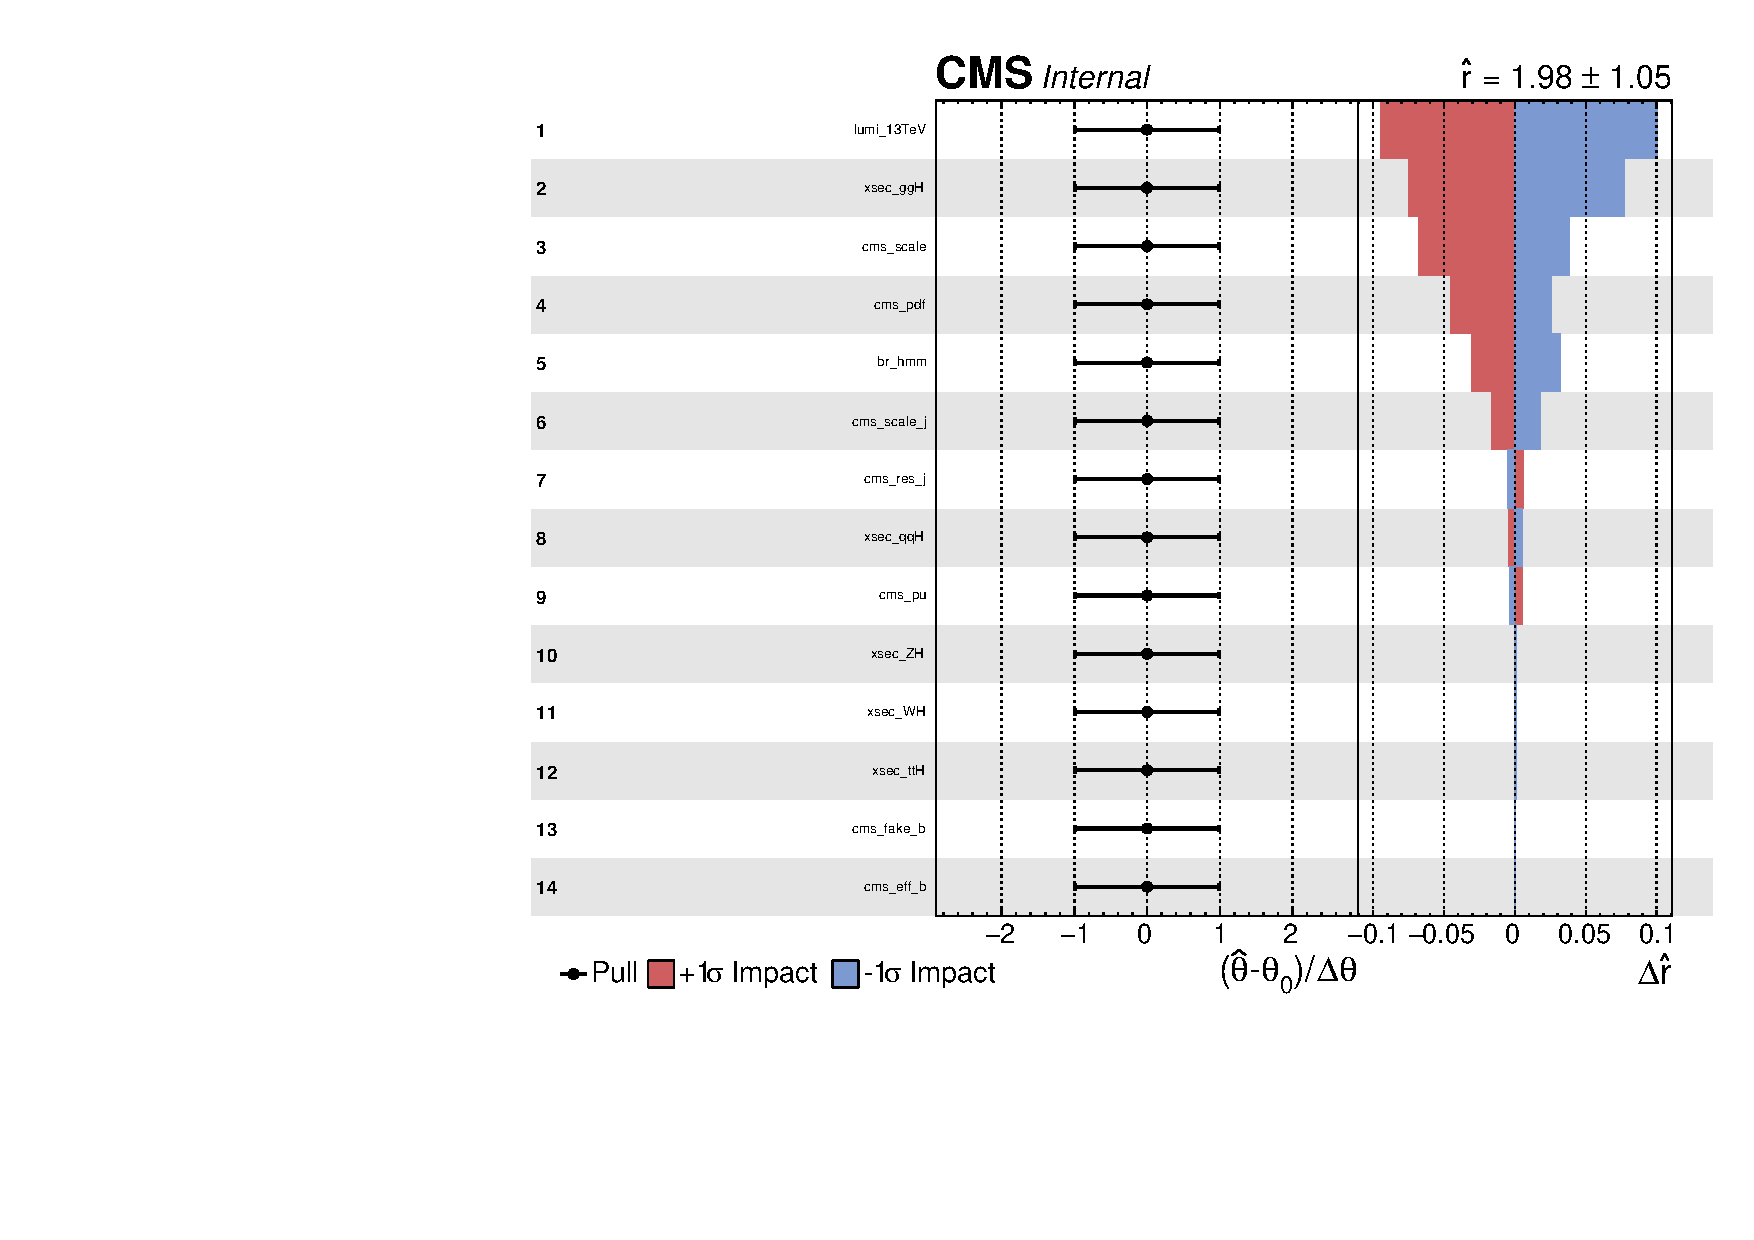
\includegraphics[width=0.631\textwidth]{figures/sig_syst/impacts.pdf}
    \caption{Impact plots derived from the Asimov dataset.}
    \label{fig:impacts}
\end{figure}

\section{Background systematic uncertainties}
\label{bkg_syst}

\subsection{Background fit function bias}
As presented in Sec.~\ref{bkg_model} we identified two classes of models to fit the background
dimuon mass spectrum, physics
motivated models and general purpose series able to describle any smoothly falling
functional forms (polynomials, sum of exponentials).

The number of fit families considered in estimating the bias induced by the choice
of the background fit function is constrained using the F-Test method at 95\% CL.

The background fit functions are normalised to the data and 1000
signal plus background toys were generated with the signal model and
a certain background model. The obtained dimuon toy mass distribution
is fit the signal plus background model where the background model
can be any of the functional forms selected with the F-test. The obtained signal strength
is compared with the injected one, here set to 1, and devided by the obtained signal strength
error. The median is used to quote the background fit function bias.

Two complete sets of bias scans in all categories at 125~GeV were conducted with independent
toys and bias machinery. These are summarised in Appendix~\ref{app:Bias}.
%The results for our most sensitive category of events are shown in Fig.~\ref{fig:cat12bias}.
The baseline background model is the perturbed
exponential times Breit-Wigner (``BWZRedux'').  The two sets of bias scans
are checked explicitly for agreement in the BWZReduz bias against Bernstein
polynomials and a sum of exponentials, with orders determined by the F-test.
The bias vs. Bernstein is indicated by the purple box, and sum of exponentials
by a black box, in the plots.

In the end, we see that the two sets of bias scans agree quite well for most
categories and pairs of fit vs. reference functions.  Some disagreements may
be due to different orders of Bernstein polynomials being chosen by the F-tests.
In c10, c8, c7, c5, c3, and c2, the Bernstein polynomial is biased against every
other function, and every other function is biased against the Bernstein polynomial.
This indicates that the Bernsteins do not characterize the data well in these
categories, so they are excluded from consideration as reference functions.
In c10 and c5, the BWZRedux bias against all other functions is less than 25\%.
In c8, c7, and c3, a function formed of the BWZRedux plus a linear term has a
bias of less than 25\% against all other functions, including the sum of exponentials.
Categories c12, c11, c6, c4, and c1 all have at least one fit function with bias
less than 20\% against all other functions.  Often this least-biased fit function
is a Bernstein, while all the other fit functions are biased against the Bernstein.
The BWZRedux function in category c9 has a 30 to 50\% bias against the Bernstein
polynomial, and in c0 has 30 to 60\% bias against the sum of exponentials.

Only in few categories will need explicit systematic uncertainties to parameterize
the the bias due to choice of fit.  In most of these categories the bias is small,
so the impact on the final limit is expected to be negligible.

%\begin{figure}
%  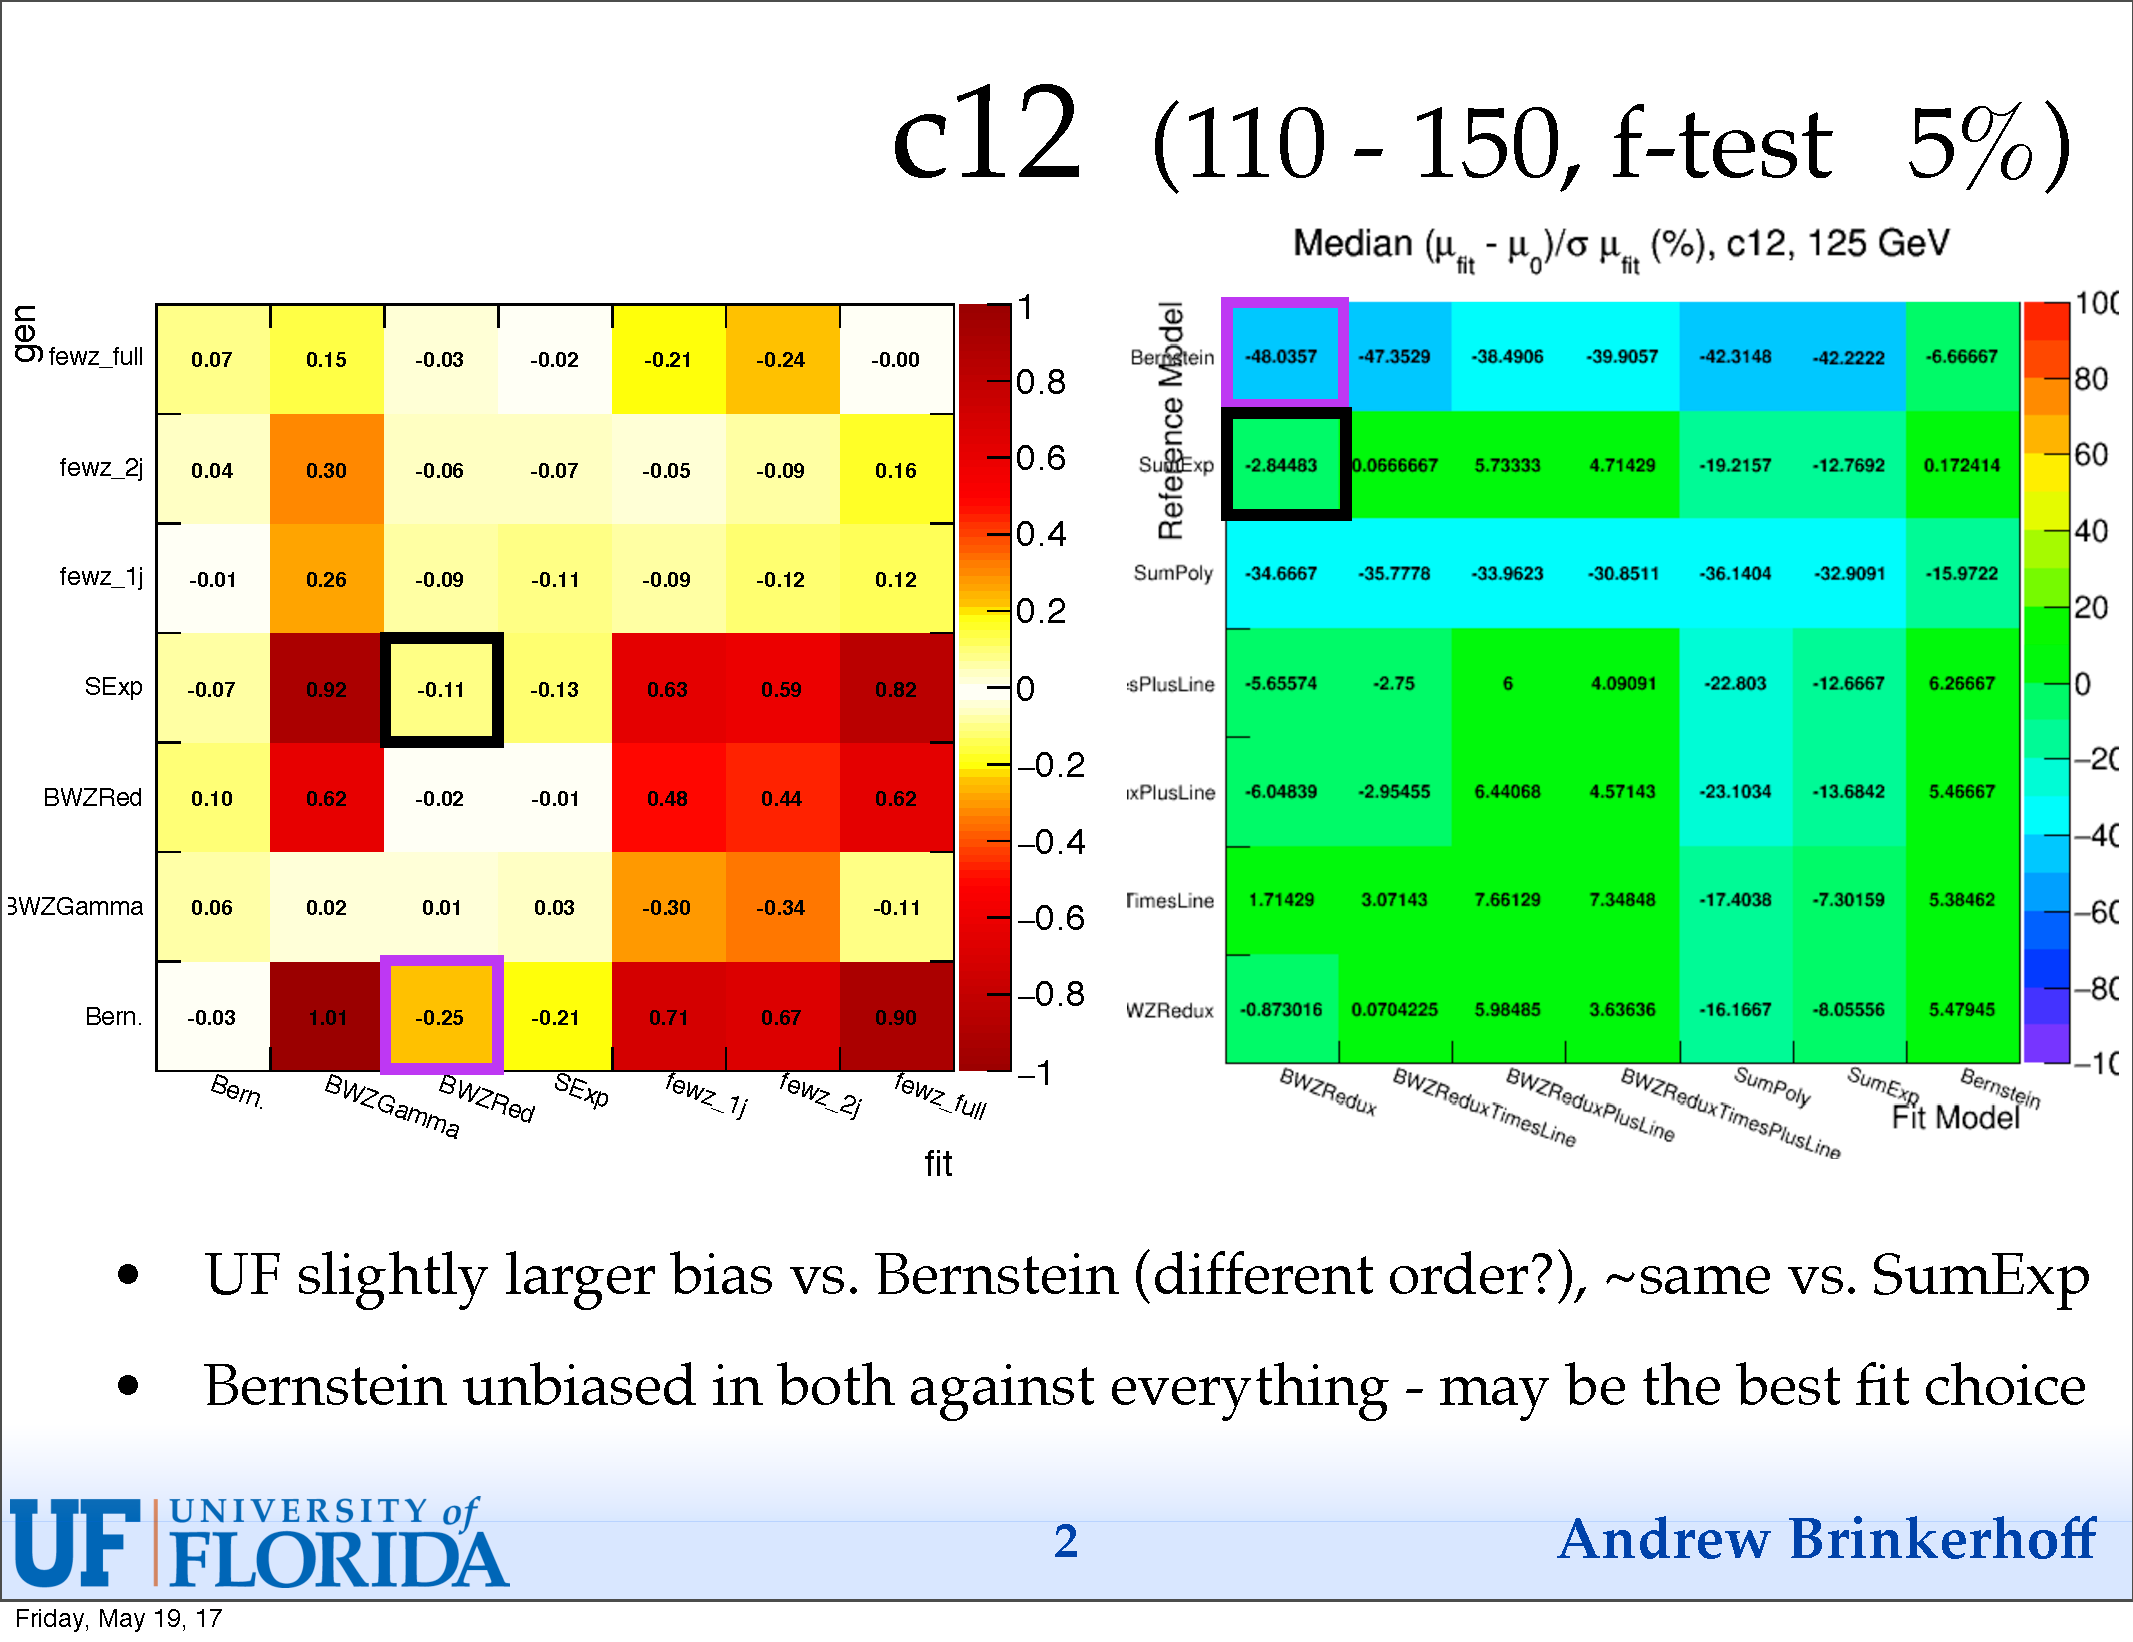
\includegraphics[width=0.8\textwidth]{figures/appendix_bias/UF_MIT_p1.pdf}
%  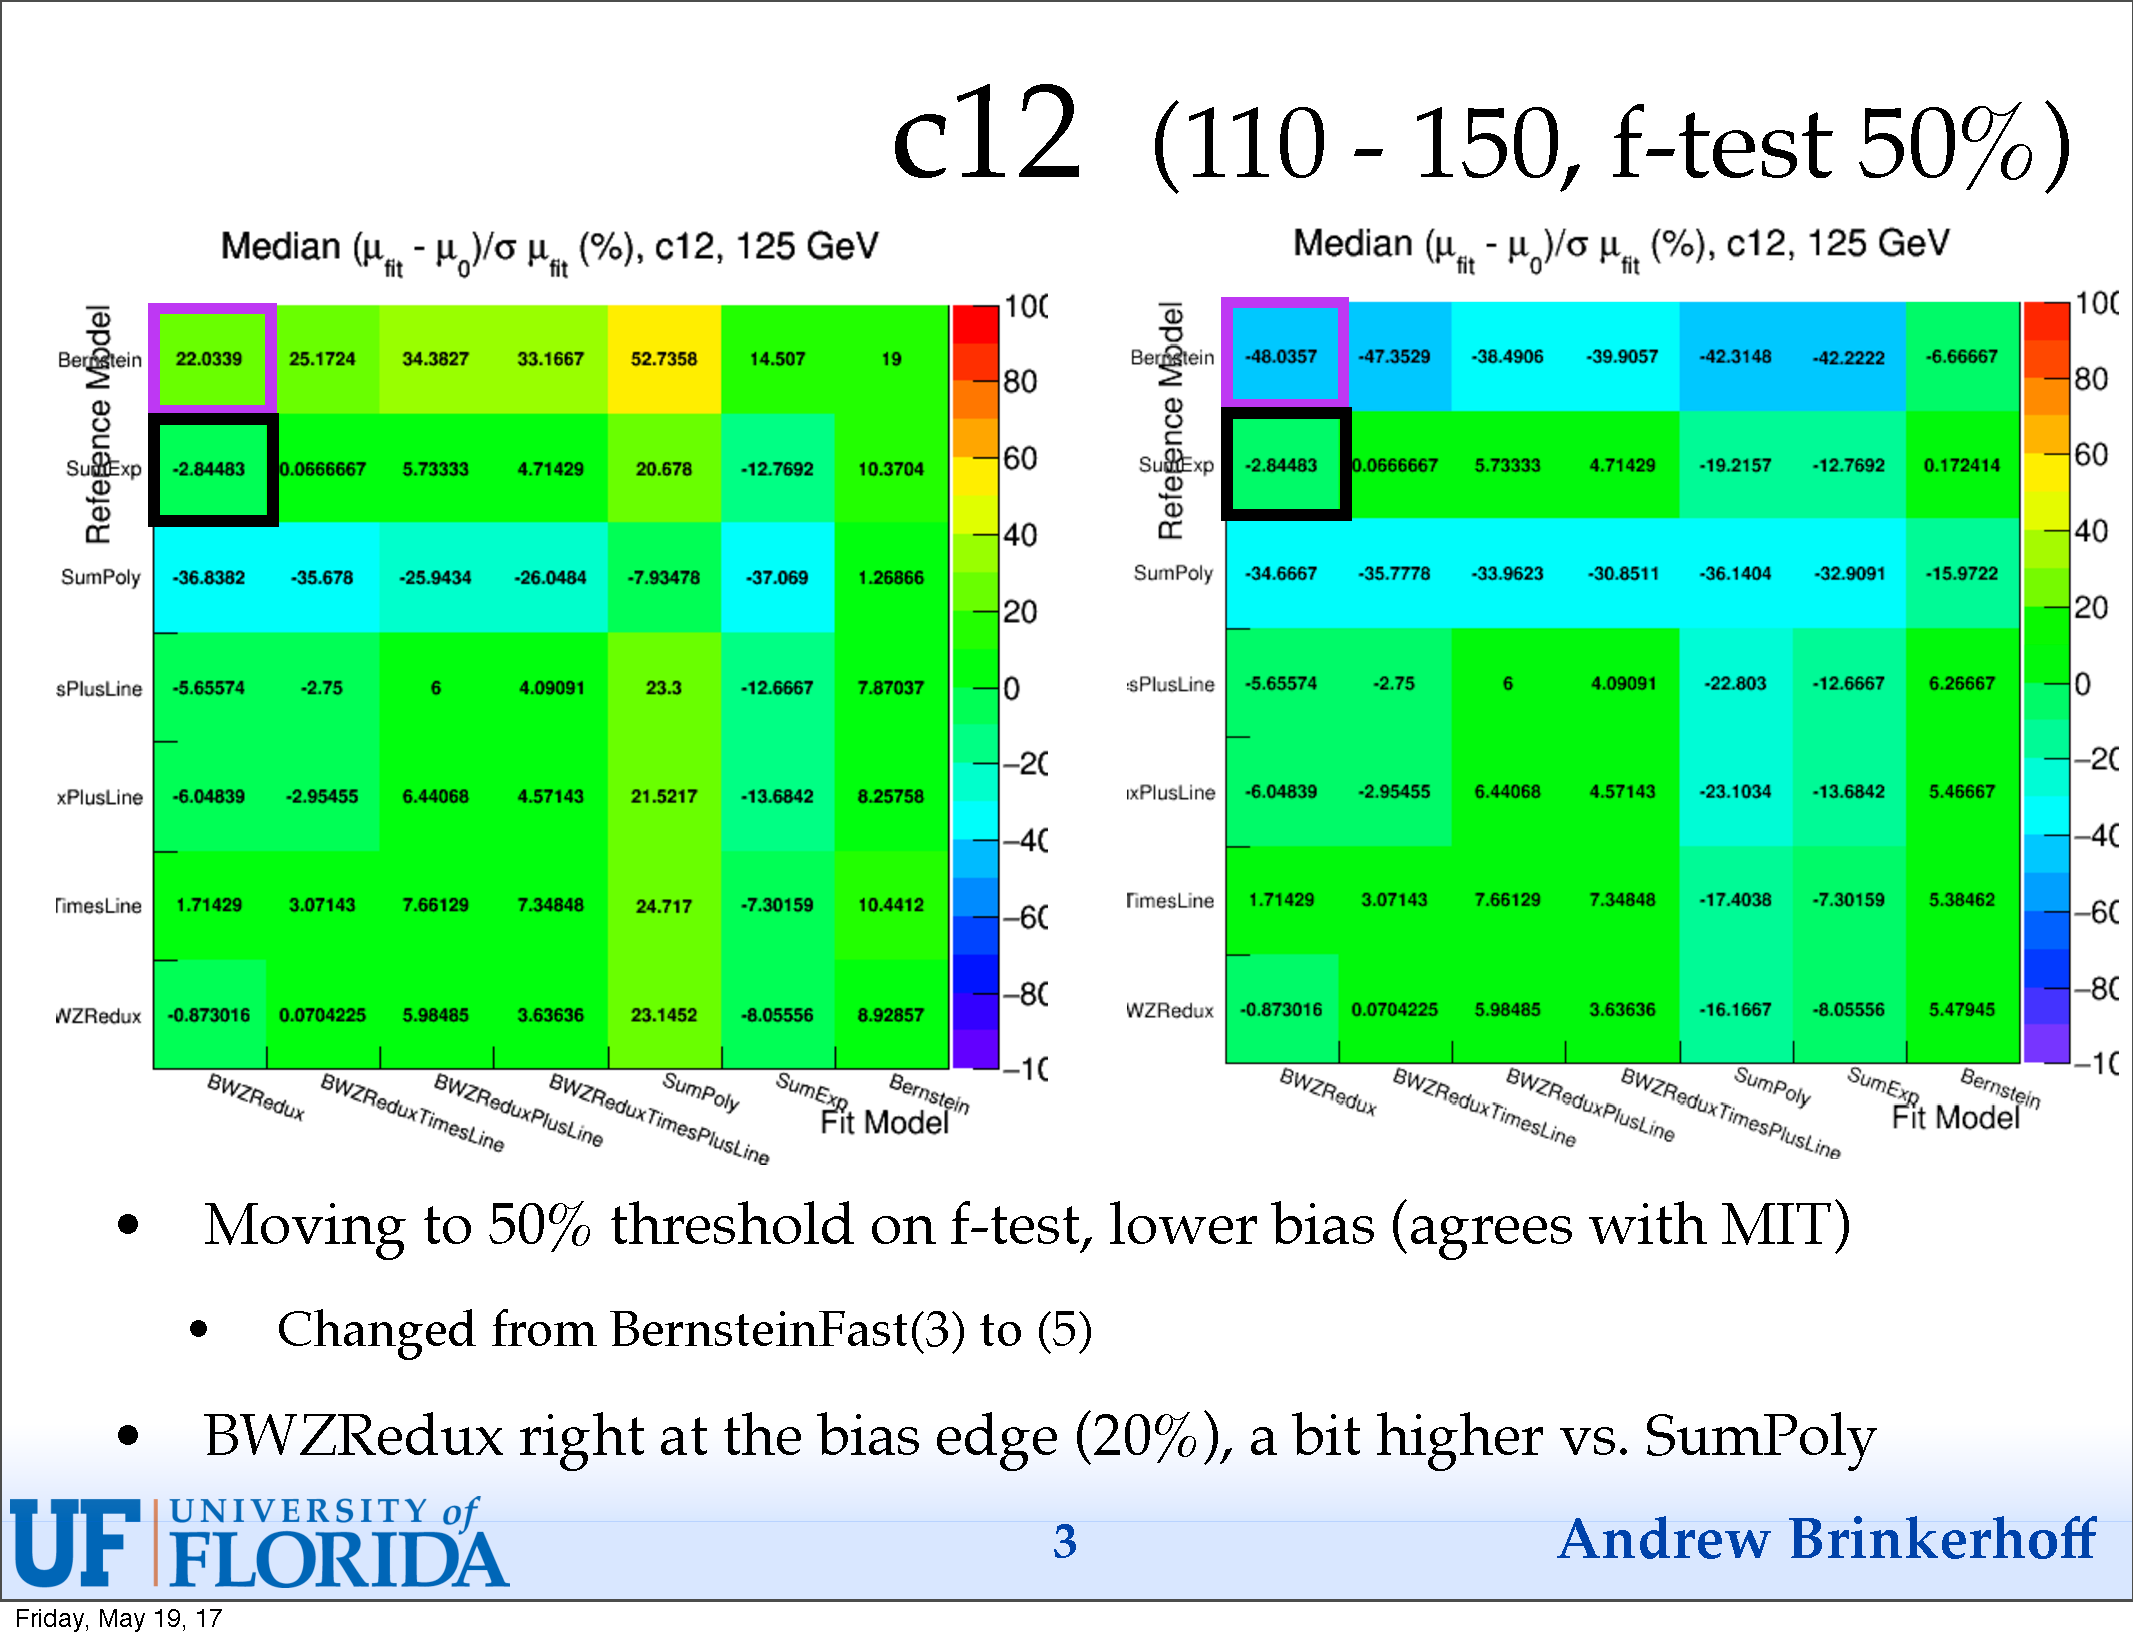
\includegraphics[width=0.8\textwidth]{figures/appendix_bias/UF_MIT_p2.pdf}
%  \label{fig:cat12bias}
%  \caption{The background fit function bias scan for the category 12 performed by MIT (left) and UF (right).}
%\end{figure}


%\subsection{Discrete profile method -- ``Envelope''}


